


\part{Extendiendo el Simulador simusched}

\section{Ejercicio 3}

Implementamos la clase requerida.

\section{Ejercicio 4}

\subsection{Lote 1}

Primero creamos un nuevo tipo de Tarea llamada TaskCPUIOCPU que recibe 3 parametros:

\begin{enumerate}
 \item n Tiempo de ejecuci\'on de CPU en ciclos de reloj
 \item i Tiempo de ejecuci\'on de IO en ciclos de reloj
 \item m Tiempo de ejecuci\'on de CPU en ciclos de reloj
\end{enumerate}

Esta tarea ejecuta en el CPU (n) se bloquea por (i) y luego sigue ejecutando (m).

\paragraph{}
Creamos el siguiente grupo de tareas \verb|ejercicio4_1.tsk|

\begin{framed}
\begin{verbatim}
# FILE ejercicio4_1.tsk
*2 TaskCPU 30
TaskCPUIOCPU 10 20 10
\end{verbatim}
\end{framed}

Luego ejecutamos Simusched con los siguientes parametros:

\begin{framed}
\begin{verbatim}
./simusched ejercicio4_1.tsk 1 SchedRR 3 | python graphsched.py > ejercicio4_1.png
\end{verbatim}
\end{framed}

\begin{figure}[h!]
  \caption{Dos tareas de uso intensivo de CPU y una tarea de tipo TaskCPUIOCPU.}
  \centering
    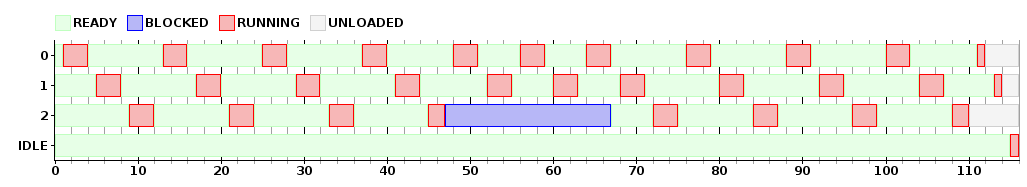
\includegraphics[width=1\textwidth]{img/ejercicio4_1.png}
\end{figure}

Se puede ver en el grafico que se van alternando los 3 procesos con un quantum de 3 unidades hasta que el proceso (2) se bloquea.

Mientras el (2) est\'a bloqueado se puede ver que los otros dos procesos van altenando su ejecuci\'on. 

Hasta que el proceso (2) se desblquea y nuevamente se vuelven a alternar los 3 procesos.

\subsection{Lote 2}

Utilizamos nuevamente la tarea que creamos anteriormente TaskCPUIOCPU.

Creamos el archivo \verb|ejercicio4_2.tsk|

\begin{framed}
\begin{verbatim}
# FILE ejercicio4_2.tsk
TaskCPUIOCPU 10 20 10
@3
TaskCPUIOCPU 15 20 5
@10
TaskCPU 10
\end{verbatim}
\end{framed}

Luego ejecutamos Simusched con los siguientes parametros:

\begin{framed}
\begin{verbatim}
./simusched ejercicio4_2.tsk 1 SchedRR 4 | python graphsched.py > ejercicio4_2.png
\end{verbatim}
\end{framed}

\begin{figure}[h!]
  \caption{Dos tareas de tipo TaskCPUIOCPU y una tarea de uso intensivo de CPU.}
  \centering
    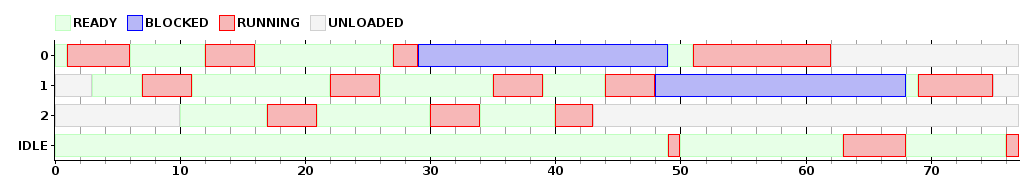
\includegraphics[width=1\textwidth]{img/ejercicio4_2.png}
\end{figure}

Hay tres procesos que se estan ejecutando.

\section{Ejercicio 5}

Implementamos la clase requerida.
